\documentclass[11pt]{article}
\usepackage{amsmath}
\usepackage{amssymb}
\usepackage{amsthm}
\usepackage{caption}
\usepackage{cleveref}
\usepackage{enumitem}
\newlist{inlinelist}{enumerate*}{1}
\setlist*[inlinelist,1]{label=(\arabic*)}
\usepackage[totalwidth=450pt, totalheight=630pt]{geometry}
\usepackage{graphicx}
\usepackage{mathrsfs}
\usepackage[round]{natbib}
\usepackage{tikz}
\usetikzlibrary{calc}
\usepackage{verbatim}
\usepackage{xcolor}
\definecolor{mid_green}{HTML}{99d8c9}

\captionsetup{width=0.8\textwidth}
\DeclareMathOperator*{\argmax}{arg\,max}

\newtheorem{corollary}{Corollary}
\newtheorem{definition}{Definition}
\newtheorem{lemma}[corollary]{Lemma}
\newtheorem{theorem}[corollary]{Theorem}

\theoremstyle{definition}
\newtheorem{example}{Example}


\setlength{\tabcolsep}{1em}
\setlist{listparindent=\parindent, parsep=0pt}
\newtheoremstyle{custom}{}{}{\itshape}{}{\bfseries}{.}{.5em}{\thmnote{#3}}
\theoremstyle{custom}
\newtheorem*{customthm}{Theorem}
\newcommand{\EE}{\mathbb{E}}
\newcommand{\PP}{\mathbb{P}}
\newcommand{\RR}{\mathbb{R}}
\newcommand{\ZZ}{\mathbb{Z}}

% Commands for inline commenting that shows up on pdf
\newcommand{\WFcomment}[1]{{\color{red}{(WF: \bf \sc #1) }}}
\newcommand{\KHcomment}[1]{{\color{green!60!black}{(KH: \bf \sc #1) }}}

\begin{document}

\title{Rank Verification for Exponential Families}
\author{Kenneth Hung \and William Fithian}
\date{\today}
\maketitle

\begin{abstract}
Many statistical experiments involve comparing multiple population groups. For example, a public opinion poll may ask which of several political candidates commands the most support, or a clinical trial may compare patient outcomes to determine the best of several treatment conditions. This article concerns the problem of {\em rank verification} --- post hoc tests of whether the ordering discovered in the data is in fact statistically significant. For exponential family models, we show under mild conditions that an unadjusted two-tailed pairwise test comparing the ``winning'' population to the ``runner-up'' is a valid test of whether the winner is truly the best. We also propose comparably simple procedures to give lower confidence bounds on the gap between the winning population and the others, and to verify ranks beyond the first.
\end{abstract}

\section{Introduction}
\label{sec:intro}

\subsection{Motivating Example: Iowa Republican Caucus Poll}
\label{sec:iowa}

\Cref{tbl:poll} shows the result of a Quinnipiac University poll asking 890 Iowa Republicans their preferred candidate for the Republican presidential nomination \citep{quinnipiac}. Donald Trump led with $31\%$ of the vote, Ted Cruz came second with $24\%$, Marco Rubio third with $17\%$, and ten other candidates including ``Don't know'' trailed behind. 

\begin{table}[htbp]
\begin{center}
\begin{tabular}{c c c c}
	\hline
	Rank & Candidate & Result & Votes \\
	\hline
	$1$ * & Trump & $31\%$ & $276$ \\
	$2$ * & Cruz & $24\%$ & $214$ \\
	$3$ * & Rubio & $17\%$ & $151$ \\
	$4$ * & Carson & $8\%$ & $71$ \\
	$5$ & Paul & $4\%$ & $36$ \\
	$6$ & Bush & $4\%$ & $36$ \\
	$7$ & Huckabee & $3\%$ & $27$ \\
	$\vdots$ & $\vdots$ & $\vdots $ & $\vdots$ \\
	\hline
\end{tabular}
\end{center}
\caption{Results from a February 1, 2016 Quinnipiac University poll of $890$ Iowa Republicans. To compute the last column (Votes), we make the simplifying assumption that the reported percentages in the third column (Result) correspond to raw vote shares among survey respondents. The asterisks indicate that the rank is verified at $0.05$-level through a step-down procedure.}
\label{tbl:poll}
\end{table}

Seeing that Trump leads this poll, several salient questions may occur to us: Is Trump really winning, and if so by how much? And analogously, is Cruz really in second, is Rubio really in third, and so on? Note that there is implicitly a problem of multiple comparisons here, because if Cruz had led the poll instead, we would be asking a different set of questions. Indeed, the selection issue appears especially pernicious due to the so-called ``winner's curse'': given that Trump leads the poll, it more likely than not overestimates his support.

Nevertheless, if we blithely ignore the selection issue, we might carry out the following analyses to answer the questions we posed before at significance level $\alpha = 0.05$. We assume for simplicity that the poll represents a simple random sample of Iowa Republicans; i.e., that the data are a multinomial sample of size $890$ and underlying probabilities $\left(\pi_{\text{Trump}}, \pi_{\text{Cruz}}, \ldots\right)$.\footnote{The reality is a bit more complicated: before releasing the data, Quinnipiac has processed it to make the reported result more representative of likely caucus-goers.}

\begin{enumerate}
\item {\em Is Trump really winning?} If Trump and Cruz were in fact tied, then Trump's share of their combined 490 votes would be distributed as $\text{Binomial}\left(490, 0.5\right)$. Because the (two-tailed) $p$-value for this pairwise test is $p = 0.006$, we reject the null and conclude that Trump is really winning.

\item {\em By how much?} Using an exact $95\%$ interval for the same binomial model, we conclude Trump has at least $7.5\%$ more support than Cruz (i.e., $\pi_{\text{Trump}} \ge 1.075 \,\pi_{\text{Cruz}}$) and also leads the other candidates by at least as much.

\item {\em Is Cruz in second, Rubio in third, etc.?} We can next compare Cruz to Rubio just as we compared Trump to Cruz (again rejecting because $214$ is significantly more than half of 365), then Rubio to Carson, and so on, continuing until we fail to reject. The first four comparisons are all significant at level $0.05$, but Paul and Bush are tied so we stop.
\end{enumerate}

Surprisingly, all of the three procedures described above are statistically valid despite their ostensibly ignoring the implicit multiple-comparisons issue. The remainder of this article is dedicated to justifying these procedures for the multinomial family and analogous procedures in other settings.

\subsection{Generic Problem Setting and Main Result}
\label{sec:probset}

Generically, we will consider data drawn from an exponential family model with density
\begin{equation}
X \sim \exp\left(\theta'x - \psi\left(\theta\right)\right) g\left(x\right),
\label{eqn:expfam}
\end{equation}
with respect to either the Lebesgue measure on $\RR^n$ or counting measure on $\ZZ^n$. We assume further that $g\left(x\right)$ is symmetric with respect to permutation, and Schur concave, a mild technical condition defined in \Cref{sec:maj}. In addition to the multinomial family, model~\eqref{eqn:expfam} also encompasses settings such as comparing independent binomial treatment outcomes in a clinical trial, competing sports teams under a Bradley--Terry model, entries of a Dirichlet distribution, and many more; see \Cref{sec:maj} for these and other examples.

We will generically use the term {\em population} to refer to the treatment group, sports team, political candidate, etc.\ represented by a given random variable $X_j$. As we will see, $\theta_j \ge \theta_k$ if and only if $X_j$ is stochastically larger than $X_k$; thus, there is a well-defined stochastic ordering of the populations that matches the ordering of the entries of $\theta$. We will refer to the population with maximal $\theta_j$ as the {\em best}, the one with maximal $X_j$ as the {\em winner}, and the one with maximal $X_j$ other than the winner as the {\em runner-up}. Following the convention in the ranking and selection literature, we assume that if there are multiple largest $\theta_j$, then one is arbitrarily marked as the best. Note that in cases where it is more interesting to ask which is the smallest population (for example, if $X_j$ is the number of patients on treatment $j$ who suffer a heart attack during a trial) we can change the variables to $-X$ and the parameters to $\theta$. 

Write the order statistics of $X$ as
$$X_{[1]} \ge X_{[2]} \ge \cdots \ge X_{[n]},$$
where $[j]$ will denote the random index for the $j$-th order statistic. Define $\theta_{[j]}$ as the entry of $\theta$ corresponding to the $j$-th order statistic of $X$ (so $\theta_{[1]}$ might {\em not} equal $\max_j \theta_j$, for example). We assume any ties between entries of $X$ are broken randomly.

In each of the above examples, there is a natural exact test we could apply to test $\theta_j=\theta_k$ for any two {\em fixed} populations $j$ and $k$. In the multinomial case, we would apply the conditional binomial test based on the combined total $X_j+X_k$ as discussed in the previous section. For the case of independent binomials we would apply Fisher's exact test, again conditioning on $X_j+X_k$. These are both examples of a generic UMPU pairwise test in which we condition on the other $n-2$ indices (notated $X_{\setminus \{j,k\}}$) and $X_j+X_k$, and reject the null if $X_j$ is outside the $\alpha/2$ and $1-\alpha/2$ quantiles of the conditional law $\mathcal{L}_{\theta_j=\theta_k}(X_j \mid X_j+X_k, X_{\setminus\{j,k\}})$, which crucially does not depend on the value of $\theta_j$ or $\theta_k$. We call this test the (two-tailed) {\em unadjusted pairwise test} since it makes no explicit adjustment for selection. Similarly, inverting this test for all values of $\theta_j-\theta_k$ yields an {\em unadjusted pairwise confidence interval}.\footnote{To avoid trivialities in the discrete case, we assume these procedures are appropriately randomized at the rejection thresholds to give exact level-$\alpha$ control.}

Generalizing the procedures described in \Cref{sec:iowa} we obtain the following:
\begin{enumerate}
\item {\em Is the winner really the best?} Carry out the unadjusted pairwise test comparing the winner to the runner-up. If the test rejects at level $\alpha$, conclude that the winner is really the best.
\item {\em By how much?} Construct the unadjusted pairwise confidence interval comparing the winner to the runner-up, and report the lower confidence bound obtained for $\theta_{[1]}-\theta_{[2]}$ if it is nonnegative, report $-\infty$ otherwise.
\item {\em Is the runner-up really the second best, etc.?} Continue by comparing the runner-up to the second-runner-up, again using the unadjusted pairwise test, and so on down the list comparing adjacent values. Stop the first time the test accepts.
\end{enumerate}
Procedure $2$ is modified above due to some technicalities; as we will see, reporting $-\infty$ is not really necessary because the bound can be improved with only a little more work.

We now state our main theorem: under a mild technical assumption, Procedures 1--3 described above are statistically valid, even accounting for the selection.
\begin{theorem}
Assume the model~\eqref{eqn:expfam} holds and $g\left(x\right)$ is a Schur-concave function. Then:
\begin{enumerate}
\item Procedure 1 has level $\alpha$ conditional on the best population not winning (otherwise an error is impossible).
\item Procedure 2 gives a conservative $1-\alpha$ lower confidence bound for $\theta_{[1]} - \max_{j \ne [1]} \theta_{j}$.
\item Procedure 3 is a conservative step-down procedure with familywise error rate (FWER) no larger than $\alpha$.
\end{enumerate}
\label{thm:main}
\end{theorem}

We define Schur-concavity and discuss its properties in \Cref{sec:maj}. Because any log-concave and symmetric function is Schur-concave, \Cref{thm:main} applies to all of the cases discussed above. The proof relies on the conditional selective-inference framework of \citet{Fithian:2014ws} combined with classical multiple-testing methods, as well as some properties of majorization and Schur-concavity.

Note that these procedures make an implicit adjustment for selection because they use two-tailed unadjusted tests. If we instead based our tests on an independent realization $X^*$, then, for example, Procedure 1 could use a right-tailed version of the unadjusted pairwise test. In the case $n = 2$, Procedure 1 amounts to a simple two-tailed test of the null hypothesis $\theta_1 = \theta_2$, and it is intuitively clear that a one-tailed test would be anti-conservative. More surprising is that, no matter how large $n$ is, Procedures 1--3 require no further adjustment beyond what is required when $n = 2$. 

\subsection{Related work}

\WFcomment{Merge this discussion with my discussion from NSF.}

Previous works construct tests comparing parameters in various families of distributions, by comparing just the winner and the runner-up. \citet{Gutmann:1987fk} tackles the question where the observations are from a location family, and the location parameters are compared. In which case, the difference of the winner and the runner-up has to pass a predetermined threshold. In contrast, a related paper by \citet{Karnnan:2009iv} discusses a scale family, comparing the scale parameters instead. Specifically, to test for the smallest variance across multiple populations, it is sufficient to test the ratio of the smallest to the second-smallest variances. \citet{Bofinger:1991hv} gives a location-scale family generated by translating an exponential distribution as well. Similarly, test the difference between the winner and the runner-up is enough. A follow-up paper by \citet{Maymin:1992fz} gave an analogous result for location-scale families, yet still under the constraints of independence.

However, as location-scale families have limited overlap with exponential families, the counterpart question for exponential families remains unaddressed. Location-scale families assumes independence between observations, while this is not necessarily the case in exponential families. For instance, in the vicinity of the polling problem above, \citet{Nettleton:2009ht} provides an asymptotic test for multinomial distribution, imposing the selection by considering intersection-union tests. \citet{Ng:2007cn} also analyzes the multinomial case for an exact test, but with an additional restriction that maximum observation is a known constant $M$. In terms of the polling problem above, we poll until one candidate hits a goal $M$. While in either papers the observations $X$ are not independent, it still suffices to test the difference between the winner and the runner-up.

One final result that has our attention is the subset selection problem \citep{Gupta:1967wg}. The procedure provided in the paper can indeed be used to solve the multinomial case. It selects a subset that contains the largest, or ``tagged'', parameter with probability $1-\alpha$. Confirming the largest parameter is thus equivalent to asserting the selected subset has size $1$. \Cref{sec:subsetsel} includes a comparison of our proposed test and their test.

\subsection{Outline}

\WFcomment{Rewrite for motivation}

\Cref{sec:maj} gives a formal definition of Schur-concavity, as well as common examples satisfying this condition. \Cref{sec:winnerbest} proves that an unadjusted pairwise test comparing the winner to the runner-up is valid, and demonstrates the power of this test. \Cref{sec:confbound,sec:stepdown} justify Procedures 2 and 3. We conclude by examining a published study with our methods in \Cref{sec:disc}.

\section{Majorization and Schur-concavity}
\label{sec:maj}

We start by reviewing the notion of {\em majorization}, defined on both $\RR^n$ and $\ZZ^n$.

\begin{definition}
For two vectors $a$ and $b$ in $\RR^n$ (or $\ZZ^n$), suppose sorting the two vectors in descending order gives
$a_{\left(1\right)} \ge \cdots \ge a_{\left(n\right)}$ and $b_{\left(1\right)} \ge \cdots \ge b_{\left(n\right)}$. We say that $a \succeq b$ ($a$ majorizes $b$) if for $1 \le i < n$,
\begin{align*}
a_{\left(1\right)} + \cdots + a_{\left(i\right)} & \ge b_{\left(1\right)} + \cdots + b_{\left(i\right)}, \quad \text{and}\\
a_{\left(1\right)} + \cdots + a_{\left(n\right)} & = b_{\left(1\right)} + \cdots + b_{\left(n\right)}.
\end{align*}
This forms a partial order in $\RR^n$ (or $\ZZ^n$).
\end{definition}

Intuitively, majorization is a partial order that monitors the evenness of a vector: the more even a vector is, the ``smaller'' it is. There are two properties of majorization that we will use in the proofs.

\begin{lemma}~\\
\begin{enumerate}
\item Suppose $\left(x_1, x_2, x_3, \ldots\right)$ and $\left(x_1, y_2, y_3, \ldots\right)$ are two vectors in $\RR^n$. Then
$$\left(x_1, x_2, x_3, \ldots\right) \succeq \left(x_1, y_2, y_3, \ldots\right) \text{ if and only if } \left(x_2, x_3, \ldots\right) \succeq \left(y_2, y_3, \ldots\right).$$
\item (Principle of transfer) If $x_1 > x_2$ and $t \ge 0$, then
$$\left(x_1 + t, x_2, x_3, \ldots\right) \succeq \left(x_1, x_2 + t, x_3, \ldots\right).$$
If $t \le 0$, the majorization is reversed.
\end{enumerate}
\label{lma:twoprop}
\end{lemma}

\begin{proof}~\\
\begin{enumerate}
\item The property follows from an equivalent formulation of majorization listed in \citet{Marshall:2010hb}, where $x \succeq y$ if and only if
$$\sum_{j=1}^n x_n = \sum_{j=1}^n y_n ~~~~ \text{ and } ~~~~ \sum_{j=1}^n \left(x_j - a\right)_+ \ge \sum_{j=1}^n \left(y_j - a\right)_+ \text{ for all } a \in \RR.$$

\item Proved in \citet{Marshall:2010hb}. \qedhere
\end{enumerate}
\end{proof}

\begin{definition}
A function $g$ is Schur-concave if $x \succeq y$ implies $g\left(x\right) \le g\left(y\right)$.
\end{definition}

A Schur-concave function is symmetric by default since $a \succeq b$ and $b \succeq a$ if and only if $b$ is a permutation of the coordinates of $a$. Conversely a symmetric and log-concave function is Schur-concave \citep{Marshall:2010hb}, thus many common exponential family distributions lie in this class. To name a few:

\begin{example}[Independent binomial treatment outcomes in a clinical trial]
 If each of $n$ different treatments are applied to $m$ patients independently, the number of positive outcomes $X_j$ for treatment $j$ is $\text{Binomial}\left(m, p_j\right)$. The best treatment would be the treatment with the highest success probability $p_j$. The joint distribution of $X$ is given by
$$p\left(x\right) \propto \exp\left(x' \left(\log p\right)\right) \frac{1}{x_1! \left(m-x_1\right)! \cdots x_n! \left(m-p_n\right)!}$$
The carrier measure above is Schur-concave.
\end{example}

\begin{example}[Competitive sports under the Bradley--Terry model]
  Suppose $n$ players compete in a round robin tournament, where player $j$ has ability $\theta_j$, and the probability of player $j$ winning against player $k$ is
$$\frac{e^{\theta_j - \theta_k}}{1 + e^{\theta_j - \theta_k}} = \frac{e^{\left(\theta_j - \theta_k\right) / 2}}{e^{\left(\theta_j - \theta_k\right) / 2} + e^{\left(\theta_k - \theta_j\right) / 2}}.$$

Let $Y_{jk}$ be an indicator for the match between player $j$ and $k$, where we take $Y_{jk} = 1$ if $j$ beats $k$ and $Y_{jk} = 0$ if $k$ beats $j$. For symmetry, we will also adopt the convention that $Y_{jk} + Y_{kj} = 1$. Thus the joint distribution of $Y=\left(Y_{jk}\right)_{j\neq k}$ is
$$p\left(y\right) \propto \exp\left(\sum_j 2\theta_j \sum_{k \ne j} y_{jk}\right)  = \exp\left(2\theta' x\right),$$
where $x_j = \sum_{k \ne j} y_{jk}$. In other words, if $X_j$ is the number of wins by player $j$, then $X=(X_1,\ldots,X_n)$ is a sufficient statistic with distribution
$$p\left(x\right) = \exp\left(2\theta' x\right) g\left(x\right),$$
where $g\left(x\right)$ is a function that counts the number of possible tournament results giving the net win vector $x$. A bijection proof shows that $x$ is indeed Schur-concave. Therefore, we can use Procedures 1--3 to compare player qualities.
\end{example}

\begin{example}[Comparing the variances of different normal populations] Suppose there are $n$ normal populations with laws $N\left(\mu_j, \sigma_j^2\right)$ and $m$ independent observations from each of them. The sample variance for population $j$ can be denoted as $R_j$. By Cochran's theorem, $\left(m-1\right) R_j \sim \sigma_j^2 \chi_{m-1}^2$, and thus the joint distribution of $R$ is
\begin{align*}
r & \sim \prod_{j=1}^n \left(\frac{\left(m-1\right) r_j}{\sigma_j^2}\right)^{\left(m-3\right) / 2} e^{-\left(m-1\right) r_j / 2 \sigma_j^2} 1_{\left\{r_j > 0 \right\}} \\
& \propto \exp\left(-\frac{m-1}{2 \sigma_1^2} r_1 - \cdots - \frac{m-1}{2 \sigma_n^2} r_n\right) \prod_{j=1}^n r_j^{\left(m-3\right) / 2} 1_{\left\{r > 0\right\}}.
\end{align*}
The carrier measure is $\prod_{j=1}^n r_j^{\left(m-3\right) / 2} 1_{\left\{r > 0\right\}}$, which is Schur-concave. Thus, we can use Procedures 1--3 to find populations with the smallest or largest variances.
\end{example}

\section{Verifying the Winner: Is the Winner Really the Best?}
\label{sec:winnerbest}

First, we justify the notion that the population with largest $\theta_j$ is also the largest population in stochastic order:
\begin{theorem}
\label{thm:stoch}
For a multivariate exponential family with a symmetric carrier distribution, $X_1 \ge X_2$ in stochastic order if and only if $\theta_1 > \theta_2$.
\end{theorem}

\begin{proof}
It suffices to prove the ``if'' part, as the ``only if'' part can be follows from swapping the role of $\theta_1$ and $\theta_2$. For any fixed $a$, and $X_1 \ge a$ and $X_2 < a$, we have $X_1 > X_2$ and
$$\exp\left(\theta_1 X_1 + \theta_2 X_2 + \cdots + \theta_n X_n - \psi\left(\theta\right)\right) g\left(X\right) \ge \exp\left(\theta_1 X_2 + \theta_2 X_1 + \cdots + \theta_n X_n - \psi\left(\theta\right)\right) g\left(X\right).$$
Integrating both sides over the region $\left\{X: X_1 \ge a, X_2 < a\right\}$ gives
$$\PP\left[X_1 \ge a, X_2 < a\right] \ge \PP\left[X_1 < a, X_2 \ge a\right].$$
Now adding $\PP\left[X_1 \ge a, X_2 \ge a\right]$ to both probabilities gives
$$\PP\left[X_1 \ge a\right] \ge \PP\left[X_2 \ge a\right],$$
meaning that $X_1$ is greater than $X_2$ in stochastic order.
\end{proof}

Before proving our main result for Procedure 1, we give the following lemma, which clarifies a key idea in the proof.

\begin{lemma}[\citealp{Berger:1982hy}]
If $p_j$ are valid $p$-values for testing null hypothesis $H_{0j}$, then $p_* = \max_j p_j$ is a valid $p$-value for the union null (i.e.\ disjunction null) hypothesis $H_0 = \bigcup_j H_{0j}$. If all the $p$-values are uniform, then $p_*$ is also a valid $p$-value.
\label{lma:union}
\end{lemma}

\begin{proof}
Under $H_0$, one of the $H_{0j}$ is true; without loss of generality assume it is $H_{01}$. Then,
$$\PP\left[p_* \le \alpha\right] \le \PP\left[p_1 \le \alpha\right] \le \alpha.$$
Therefore $p_*$ is a valid $p$-value for the union null hypothesis.
\end{proof}

We are now ready to prove our result for Procedure 1, restated here for reference.

\begin{customthm}[Part 1 of \Cref{thm:main}]
Assume the model~\eqref{eqn:expfam} holds and $g\left(x\right)$ is a Schur-concave function. Procedure 1 (the unadjusted pairwise test) has level $\alpha$ conditional on the best population not winning.
\end{customthm}

\begin{proof}
Let $j^*$ denote the (fixed) index of the best population, so $\theta_{j^*} \geq \max_{j\neq j^*} \theta_j$. The type I error --- the probability of incorrectly declaring any other $j$ to be the best --- is
$$\PP\left[\bigcup_{j \ne j^*} \text{declare } j \text{ best}\right] \le \sum_{j \ne j^*} \PP\left[\text{declare } j \text{ best} \;\middle|\; j \text{ wins}\right] \PP\left[j \text{ wins}\right],$$
recalling that ties are broken randomly, so there is only one winner in any realization. Thus, it is enough to bound $\PP_{\theta}\left[ \text{declare } j \text{ best} \;\middle|\; j \text{ wins}\right] \leq \alpha$, for each $j \ne j^*$, and for all $\theta$ with $j^* \in \argmax_j \theta_j$. Then we will have
\begin{equation}
\PP\left[\bigcup_{j \ne j^*} \text{declare } j \text{ best}\right] \le \sum_{j \ne j^*} \alpha \cdot \PP\left[j \text{ wins}\right] \le \frac{n-1}{n} \alpha,
\label{eq:marginal}
\end{equation}
where the second inequality uses the stochastic ordering on $X_j$. \WFcomment{Should we put that Prop. first? Also I'm not sure it quite justifies the second inequality.}

We start by assuming that we are working with the Lebesgue measure rather than the counting measure (eliminating the possibility of ties). The necessary modification of the proof for the counting measure case is provided at the end of this proof.

To minimize notational clutter, we consider only the case where the winner is $1$ and the runner-up is $2$, etc., i.e.\ $X_1 \ge \cdots \ge X_n$. For other cases, the following proof remains valid under relabeling and can thus be applied. In this case, we will test the null hypothesis $H_{01}: \theta_1 \le \max_{j > 1} \theta_j$, which is the union of the null hypotheses $H_{01j}: \theta_1 \le \theta_j$ for $j \ge 2$. For each of these we can construct an exact $p$-value $p_{1j}$, which is valid under $H_{01j}$ conditional on $A_1$, the event that $X_1$ is the winner. Hence by \Cref{lma:union}, a test that rejects when $p_{1*} = \max_j p_{1j} \leq \alpha$ is valid for $H_{01}$ conditional on $A_1$. Procedure 1 performs an unadjusted pairwise test comparing $X_1$ to $X_2$. Hence it is sufficient to show that $p_{12} = p_{1*}$ and that rejecting when $p_{12}\leq \alpha$ coincides with the unadjusted pairwise test.

Our proof has three main parts:
\begin{inlinelist}
\item deriving $p_{1j}$ for each $j\ge 2$,
\item showing that $p_{12} \ge p_{1j}$ for each $j\ge 2$, and
\item showing that $p_{12}$ is an unadjusted pairwise $p$-value.
\end{inlinelist}

\paragraph{Derivation of $p_{1j}$}

Following the framework in \citet{Fithian:2014ws}, we first construct the p-values by conditioning on the selection event where the winner is $1$: 
$$A_1 = \left\{X_1 \ge \max_{j > 1} X_j\right\}.$$
For convenience, we let
$$D_{jk} = \frac{X_j - X_k}{2} ~~~~ \text{ and } ~~~~ M_{jk} = \frac{X_j + X_k}{2}.$$

We then re-parametrize to replace $X_1$ and $X_j$ with $D_{1j}$ and $M_{1j}$. The distribution is now an exponential family with sufficient statistics $D_{1j}, M_{1j}, X_{\setminus\left\{1, j\right\}}$ and corresponding natural parameters $\theta_1 - \theta_j, \theta_1 + \theta_j, \theta_{\setminus\left\{1, j\right\}}$. We now consider
\begin{equation}
\mathcal{L}_{\theta_1 - \theta_j = 0} \left(D_{1j} \;\middle|\; M_{1j}, X_{\setminus\left\{1, j\right\}}, A_1\right).
\label{eqn:condlaw}
\end{equation}
We can rewrite the selection event in terms of our new parameterization as
\begin{align*}
A_1 &= \left\{X_1 \ge X_j\right\} \cap \left\{X_1 \ge \max_{k \neq 1,j} X_k\right\}\\
&= \left\{D_{1j} \ge 0\right\} \cap \left\{D_{1j} \ge \max_{k \ne 1, j} X_k - M_{1j}\right\}.
\end{align*}
The conditional law in \Cref{eqn:condlaw}, in particular, is a truncated distribution
\begin{align*}
p\left(D_{1j} \mid \cdots\right) & \propto \exp\left(\left(\theta_1 - \theta_j\right) D_{1j} + \theta_2 X_2 + \cdots + \left(\theta_1 + \theta_j\right) M_{1j} + \cdots + \theta_n X_n \right) \\
& ~~~~~~~~ g\left(M_{ij} + D_{ij}, X_2, \ldots, M_{ij} - D_{ij}, \ldots X_n\right) 1_{A_1} \\
& \stackrel{\text{(a)}}{\propto} g\left(M_{ij} + D_{ij}, X_2, \ldots, M_{ij} - D_{ij}, \ldots X_n\right) 1_{A_1},
\end{align*}
\WFcomment{This notation is confusing because there should also be another indicator that $M_{ij}=m_{ij}$ where $m_{ij}$ is the realized value this time, also for $X_{\setminus\left\{1,j\right\}}=x_{\cdots}$.}
where at step (a), conditioning on $X_{\setminus\left\{1, j\right\}}$ and $M_{1j}$ removes dependence on $\theta_{\setminus\left\{1, j\right\}}$ and $\theta_1 + \theta_j$ respectively, while $\theta_1 - \theta_j$ is taken to be $0$ under our null hypothesis.

The $p$-value for $H_{01j}$ is thus
\begin{equation}
p_{1j} = \frac{\int_{D_{1j}}^\infty g\left(M_{1j} + z, X_2, \ldots, M_{1j} - z, \ldots, X_n\right) \,dz}{\int_{\max\left\{X_2 - M_{1j}, 0\right\}}^\infty g\left(M_{1j} + z, X_2, \ldots, M_{1j} - z, \ldots, X_n\right) \,dz}.
\label{eqn:p1j}
\end{equation}

Finally, by construction, $p_{1j}$ satisfies
$$\PP_{H_{01j}}\left[p_{1j} < \alpha \;\middle|\; M_{1j}, X_{\setminus\left\{1, j\right\}}, A_1\right] \le \alpha,$$
almost surely. Marginalizing over $M_{1j}, X_{\setminus\left\{1, j\right\}}$,
$$\PP_{H_{01j}}\left[p_{1j} < \alpha \;\middle|\; A_1\right] \le \alpha.$$
Therefore these $p_{1j}$ are indeed valid $p$-values.

\paragraph{Demonstration that $p_{1*}=p_{12}$}

We now proceed to show that $p_{12}$, the $p$-value comparing the winner to the runner-up, is the largest of all $p_{1j}$. Without loss of generality, it is sufficient to show that $p_{12} \ge p_{13}$.

From the first part of this proof, both p-values are constructed by conditioning on $X_4, \ldots, X_n$. Upon conditioning these, $\left(X_1, X_2, X_3\right)$ follows an exponential family distribution, with carrier distribution
$$g_{X_4, \ldots, X_n}\left(X_1, X_2, X_3\right) = g\left(X_1, \ldots, X_n\right).$$
\WFcomment{What does the subscripting mean?}
The first point in \Cref{lma:twoprop} says that the function $g_{X_4, \ldots, X_n}$ is Schur-concave as well. We have reduced the problem to the case when $n = 3$: we can apply the result for $n = 3$ to $g_{X_4, \ldots, X_n}$ to yield $p_{12} \ge p_{13}$ for $n > 3$.

We have reduced to the case when $n = 3$. The p-values thus are
\begin{align*}
p_{12} & = \frac{\int_{D_{12}}^\infty g\left(M_{12} + z, M_{12} - z, X_3\right) \,dz}{\int_0^\infty g\left(M_{12} + z, M_{12} - z, X_3\right) \,dz}, \\
p_{13} & = \frac{\int_{D_{13}}^\infty g\left(M_{13} + z, X_2, M_{13} - z\right) \,dz}{\int_{\max\left\{X_2 - M_{13}, 0\right\}}^\infty g\left(M_{13} + z, X_2, M_{13} - z\right) \,dz}
\end{align*}

The maximum in the denominator of $p_{13}$ prompts us to consider two separate cases. First, we suppose $X_2 < M_{13}$. Changing variables such that the lower limits of both integrals in the numerator are $0$, we can re-parametrize the integrals above to give
\begin{align*}
p_{12} & = \frac{\int_0^\infty g\left(X_1 + z, X_2 - z, X_3\right) \,dz}{\int_0^\infty g\left(M_{12} + z, M_{12} - z, X_3\right) \,dz} \\
& = \frac{\int_0^\infty g\left(X_1 + z, X_2 - z, X_3\right) \,dz}{\int_{-D_{12}}^\infty g\left(X_1 + z, X_2 - z, X_3\right) \,dz}, \\
p_{13} & = \frac{\int_0^\infty g\left(X_1 + z, X_2, X_3 - z\right) \,dz}{\int_0^\infty g\left(M_{13} + z, X_2, M_{13} - z\right) \,dz} \\
& = \frac{\int_0^\infty g\left(X_1 + z, X_2, X_3 - z\right) \,dz}{\int_{-D_{13}}^\infty g\left(X_1 + z, X_2, X_3 - z\right) \,dz}.
\end{align*}
To help see the re-parametrization, each of these integrals can be thought of in terms of integrals along segments and rays. For example $p_{12}$ can be represented in terms of integrals $A$ and $B$ in \Cref{fig:p-value}. Specifically,
$$p_{12} = \frac{B}{A + B}$$

\begin{figure}[htbp]
\begin{center}
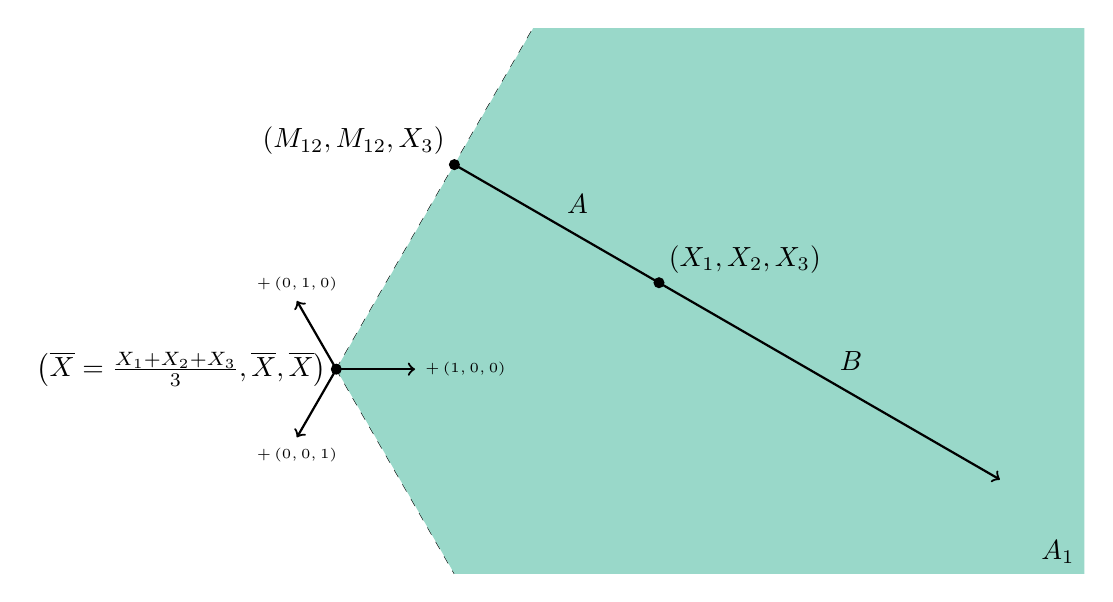
\begin{tikzpicture}
	\coordinate (C1) at (60:5);
	\coordinate (C2) at (300:3);
	\coordinate (A) at (60:3);
	\coordinate (B) at ($(A) + (330:3)$);
	\draw[dashed] (0, 0) -- (C1);
	\draw[dashed] (0, 0) -- (C2);
	\fill[mid_green] (0, 0) -- (C1) -- ($(C1) + (7, 0)$) -- ($(C2) + (8, 0)$) -- (C2) -- cycle;
	\node[above left] at ($(C2) + (8, 0)$) {$A_1$};
	\draw[thick] (A) -- (B) node[midway, above right] {$A$};
	\draw[thick, ->] (B) -- ++(330:5) node[midway, above right] {$B$};
	\fill (A) circle(2pt) node[above left] {$\left(M_{12}, M_{12}, X_3\right)$};
	\fill (B) circle(2pt) node[above right] {$\left(X_1, X_2, X_3\right)$};
	\fill (0, 0) circle(2pt) node[left] {$\left(\overline{X} = \frac{X_1 + X_2 + X_3}{3}, \overline{X}, \overline{X}\right)$};
	\draw[thick, ->] (0, 0) -- (1, 0) node[right] {\tiny $+ \left(1, 0, 0\right)$};
	\draw[thick, ->] (0, 0) -- (120:1) node[above] {\tiny $+ \left(0, 1, 0\right)$};
	\draw[thick, ->] (0, 0) -- (240:1) node[below] {\tiny $+ \left(0, 0, 1\right)$};
\end{tikzpicture}
\end{center}
\caption{The $p$-value $p_{12}$ can be written in terms of integral $A$ along the segment and $B$ along the ray. The diagram is drawn a level set of $x_1 + x_2 + x_3$. The green region represents the selection event $A_1$.}
\label{fig:p-value}
\end{figure}

\Cref{fig:compare_rays} has both the $p$-values shown on the same diagram. Proving $p_{12} \ge p_{13}$ is the same as proving
$$\frac{B}{A+B} \ge \frac{D}{C+D} ~~~~ \Longleftrightarrow ~~~~ \frac{B}{A} \ge \frac{D}{C}.$$
We will prove so by extending $A$ to include $\tilde{A}$ on the diagram. We denote the sum $A + \tilde{A}$ as $A'$. Formally,
\begin{equation}
A' = \int_{-D_{13}}^0 g\left(X_1 + z, X_2 - z, X_3\right) \,dz \ge \int_{-D_{12}}^0 g\left(X_1 + z, X_2 - z, X_3\right) \,dz = A.
\label{eqn:int_extension}
\end{equation}
It is thus sufficient to show that $B \ge D$ and $C \ge A'$.

\begin{figure}[htbp]
\begin{center}
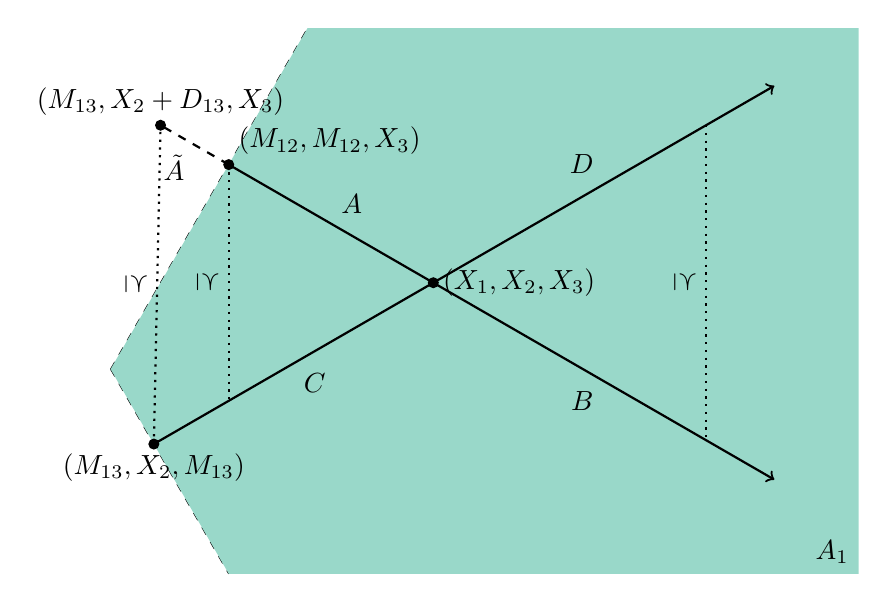
\begin{tikzpicture}
	\coordinate (C1) at (60:5);
	\coordinate (C2) at (300:3);
	\coordinate (A) at (60:3);
	\coordinate (B) at ($(A) + (330:3)$);
	\coordinate (C) at ($(0, 0)!(B)!(C2)$);
	\coordinate (D) at ($(A) + (150:1)$);
	\draw[dashed] (0, 0) -- (C1);
	\draw[dashed] (0, 0) -- (C2);
	\fill[mid_green] (0, 0) -- (C1) -- ($(C1) + (7, 0)$) -- ($(C2) + (8, 0)$) -- (C2) -- cycle;
	\node[above left] at ($(C2) + (8, 0)$) {$A_1$};
	\draw[thick] (A) -- (B) node[midway, above right] {$A$};
	\draw[thick, ->] (B) -- ++(330:5) node[midway, below left] {$B$};
	\fill (A) circle(2pt) node[above right] {$\left(M_{12}, M_{12}, X_3\right)$};
	\fill (B) circle(2pt) node[right] {$\left(X_1, X_2, X_3\right)$};
	\draw[thick] (C) -- (B) node[midway, below right] {$C$};
	\node[below] at (C) {$\left(M_{13}, X_2, M_{13}\right)$};
	\draw[thick, ->] (B) -- ++(30:5) node[midway, above left] {$D$};
	\fill ($(0, 0)!(B)!(C2)$) circle(2pt);
	\draw[thick, dashed] (A) -- (D) node[midway, below left] {$\tilde{A}$};
	\fill (D) circle(2pt) node[above] {$\left(M_{13}, X_2 + D_{13}, X_3\right)$};
	\draw[thick, dotted] (C) -- (D) node[midway, below, rotate=-90] {$\succeq$};
	\draw[thick, dotted] (A) -- ++(0, -3) node[midway, below, rotate=-90] {$\succeq$};
	\draw[thick, dotted] ($(B) + (30:4)$) -- ($(B) + (330:4)$) node[midway, below, rotate=-90] {$\succeq$};
\end{tikzpicture}
\end{center}
\caption{The $p$-value $p_{12}$ can be written in terms of integral $A$ along the segment and $B$ along the ray; and $p_{13}$ in terms of $C$ and $D$. $A'$ would refer to the sum of $A$ with the dashed line portion labeled as $\tilde{A}$, formally explained in \Cref{eqn:int_extension}. The majorization relation is indicated by the dotted line.}
\label{fig:compare_rays}
\end{figure}

Indeed from the second point in \Cref{lma:twoprop} we have
$$\left(X_1 + z, X_2 - z, X_3\right) \succeq \left(X_1 + z, X_2, X_3 - z\right)$$
for $z \le 0$ and the majorization reversed for $z \ge 0$. This majorization relation is indicated as the dotted line in \Cref{fig:compare_rays}. So Schur-concavity shows that
$$g\left(X_1 + z, X_2 - z, X_3\right) \le g\left(X_1 + z, X_2, X_3 - z\right)$$
for $z \le 0$, and the inequality reversed for $z \ge 0$. Taking integrals on both sides yields the desired inequality.

For the second case where $X_2 \ge M_{13}$, the segment $C$ will reach the line $x_1 = x_2$ first before it reaches $x_1 = x_3$, ending at $\left(X_2, X_2, X_1 - X_2 + X_3\right)$ instead. But we can still extend $A$ by $\tilde{A}$ to $\left(X_2, X_1, X_3\right)$. The rest of the proof follows. In either cases, $p_{12} \ge p_{13}$, or in generality, $p_{12} \ge p_{1j}$ for $j > 1$. In other words, $p_{12} = p_{1*}$.

\paragraph{$p_{12}$ is an unadjusted pairwise $p$-value}

Before conditioning on $A_1$, the distribution in \label{eqn:condlaw} is symmetric around 0 under $\theta_1=\theta_j$. Since the denominator of $p_{12}$ integrates over half of this symmetric distribution, it is always equal to $1/2$. Thus, the one-sided conditional test at level $\alpha$ is equivalent to the one-sided unadjusted test at level $\alpha/2$, or equivalently the two-sided unadjusted pairwise test at level $\alpha$.

\paragraph{Modification for counting measure}

Now suppose the exponential family is defined on the counting measure instead. If ties are broken independently and randomly, the end points on the rays can be considered as ``half an atom'' if the coordinates are integers (or a smaller fraction of an atom in case of a multi-way tie). The number of atoms on each ray is the same (after the extension $\tilde{A}$) and the atoms on each ray can be paired up in exactly the same way as illustrated in Figure~\ref{fig:compare_rays}, with the inequalities above still holding for each pair of the atoms. Summing these inequalities yields our desired result.
\end{proof}


\subsection{Power Comparison in the Multinomial Case}
\label{sec:subsetsel}

As the construction of this test follows \citet{Fithian:2014ws}, it uses UMPU selective level-$\alpha$ tests for the pairwise $p$-values. This section compares the power of our procedure to the best previously known method for verifying multinomial ranks, by \citet{Gupta:1967wg}. They devise a rule to select a subset that includes the maximum $\pi_j$. In other words, if the selected subset is $J\left(X\right)$, it guarantees
\begin{equation}\label{eq:subsetsel}
\PP\left[\argmax_j \pi_j \in J\left(X\right)\right] \ge 1 - \alpha.
\end{equation}
This is achieved by finding an integer $d$, as a function on $m$, $n$ and $\alpha$, and selecting the subset
$$J\left(X\right) = \left\{j: X_j \ge \max_k X_k - d\right\}.$$
We take $d(m, n, \alpha)$ to be the smallest integer such that \eqref{eq:subsetsel} holds for any $\pi$; \citet{Gupta:1967wg} provide an algorithm for determining $d$.

Subset selection is closely related to testing whether the winner is the best. In particular, we can define a test that declares $j$ the best whenever $J\left(X\right) = \left\{j\right\}$. If $J\left(X\right)$ satisfies \eqref{eq:subsetsel}, this test is valid at level $\alpha$. We next compare the power of the resulting test against the power of our Procedure 1 in a multinomial example with $\pi \propto \left(e^\delta, 1, \ldots, 1\right)$, for several combinations of $m$ and $n$.

\Cref{fig:power} gives the power curves for $\text{Multinomial}\left(m, \pi\right)$ and
$$\pi \propto \left(e^\delta, 1, \ldots, 1\right),$$
for various combinations of $m$ and $n$. For their method, we use $\alpha = 0.05$; but in light of the extra factor of $\frac{n-1}{n}$ in \eqref{eq:marginal}, we will apply the selective procedure with $\frac{n}{n-1} \alpha$ such that the marginal type I error rate of both procedures are controlled at $\alpha$. Their test coincides with our test at $n = 2$; however as $n$ grows, the selective test shows significantly more power than \citeauthor{Gupta:1967wg}'s test.

\begin{figure}[htbp]
\begin{center}
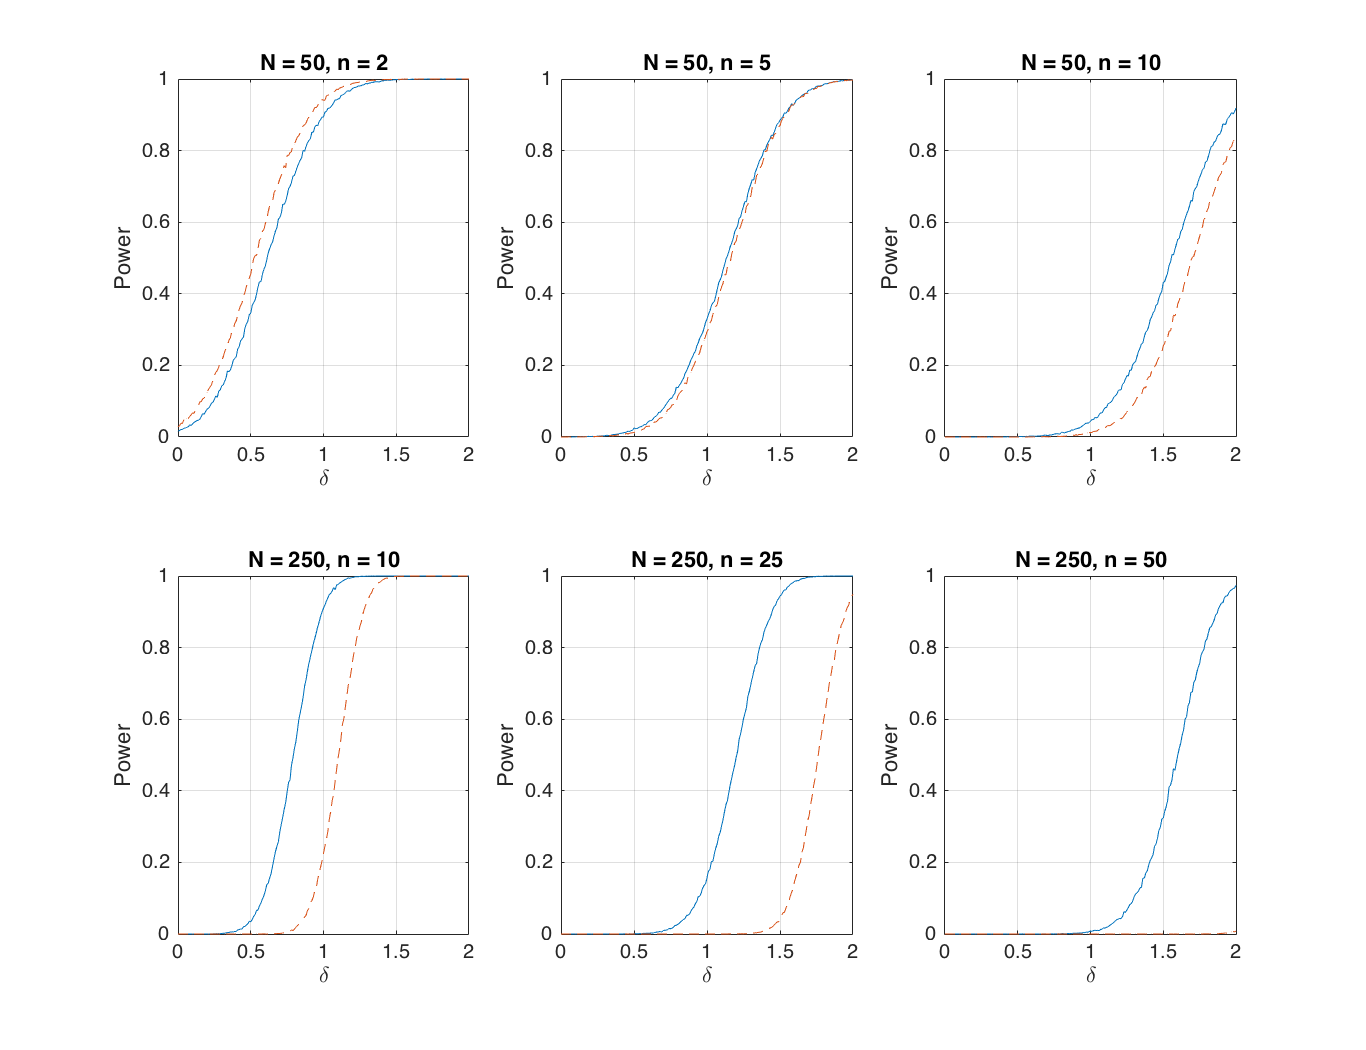
\includegraphics[width = \textwidth]{plotMultinomialPower}
\end{center}
\caption{Power curves as a function of $\delta$. The plots in the first row all have $m = 50$ and the second row $m = 250$. The solid line and the dashed line are the power for the selective test and Gupta and Nagel's test, respectively.}
\label{fig:power}
\end{figure}

To interpret, e.g., the upper right panel of Figure~\ref{fig:power}, suppose that in a poll of $m = 50$ respondents, one candidate enjoys $30\%$ support and the other $n - 1 = 9$ split the remainder ($\delta = \log\frac{0.3}{0.7 / 9} \approx 1.35$). Then our procedure has power approximately $0.3$ to detect the best candidate, while \citeauthor{Gupta:1967wg}'s procedure has power around $0.1$.

To understand why our method is more powerful, note that both procedures operate by comparing $X_{[1]}-X_{[2]}$ to some threshold, but the two methods differ in how that threshold is determined. The threshold from \citet{Gupta:1967wg} is fixed and depends on $m$ and $n$ alone, whereas in our procedure the threshold depends on $X_{[1]}+X_{[2]}$, a data-adaptive choice. 

The difference between the two methods is amplified when $n$ is large and $\pi_{[1]} \ll 1/2$. In that case, $d$ from \citeauthor{Gupta:1967wg} is usually computed based on the worst-case scenario $\pi = \left(\frac{1}{2}, \frac{1}{2}, 0, \ldots, 0\right)$; i.e. $d$ is the upper $\alpha$ quantile of
$$X_1 - X_2 \sim m - 2 \cdot \text{Binomial}\left(m, \frac{1}{2}\right) \approx \text{Normal}\left(0, m\right).$$
Thus $d \approx \sqrt{m} z_\alpha$, where $z_\alpha$ is the upper $\alpha$ quantile of a standard Gaussian. On the other hand, our method defines a threshold based on the upper $\frac{n}{n-1} \cdot \frac{\alpha}{2}$ quantile of
$$X_1 - X_2 \mid X_1 + X_2 \sim X_1 + X_2 - 2 \cdot \text{Binomial}\left(X_1 + X_2, \frac{1}{2}\right),$$
which is approximately $\sqrt{X_1 + X_2} z_{\alpha / 2}$. If $\pi_{[1]} \ll 1/2$ then with high probability $X_1 + X_2 \ll  m$, making our test much more liberal.

\section{Confidence Bounds on Differences: By How Much?}
\label{sec:confbound}

By generalizing the above, we can construct a lower confidence bound for $\theta_{[1]} - \max_{j \ne [1]} \theta_{j}$. Here we provide a more powerful Procedure 2' first. We will proceed by inverting a statistical test of the hypothesis $H_{0[1]}^\delta:\; \theta_{[1]} - \max_{j \ne [1]} \theta_{j} \le \delta$, which can be written as a union of null hypotheses:
$$H_{0[1]}^\delta = \bigcup_{j \ne [1]} H_{0[1]j}: \theta_{[1]} - \theta_j \le \delta.$$
By \Cref{lma:union}, we can construct selective exact one-tailed $p$-values $p_{[1]j}^\delta$ for each of these by conditioning on $A_{[1]}$, $M_{[1]j}$ and $X_{\setminus\left\{[1], j\right\}}$, giving us an exact test for $H_{0[1]}$ by rejecting whenever $\max_{j \ne [1]} p_{[1]j}^\delta < \alpha$.

\begin{theorem}
The $p$-values constructed above satisfy $p_{[1][2]}^\delta \ge p_{[1]j}^\delta$ for any $j \ne [1]$.
\end{theorem}

\begin{proof}
Again we start with assuming $X_1 \ge \cdots \ge X_n$. The $p$-values in question are derived from the conditional law
$$\mathcal{L}_{\theta_1 - \theta_j = \delta} \left(D_{1j} \;\middle|\; M_{1j}, X_2, \ldots, X_n, A\right),$$
which is the truncated distribution
\begin{align*}
p\left(D_{1j}\right) & \propto \exp\left(\left(\theta_1 - \theta_j\right) D_{1j} + \theta_2 X_2 + \cdots + \left(\theta_1 + \theta_j\right) M_{1j} + \cdots + \theta_n X_n \right) \\
& ~~~~~~~~ g\left(M_{1j} + D_{1j}, X_2, \ldots, M_{1j} - D_{1j}, \ldots X_n\right) 1_{A_1} \\
& \propto \exp\left(\delta D_{1j}\right) g\left(M_{1j} + D_{1j}, X_2, \ldots, M_{1j} - D_{1j}, \ldots X_n\right) 1_{A_1}.
\end{align*}

The $p$-values thus are
$$p_{1j}^\delta = \frac{\int_{D_{1j}}^\infty \exp\left(\delta z\right) g\left(M_{1j} + z, X_2, \ldots, M_{1j} - z, \ldots, X_n\right) \,dz}{\int_{\max\left\{X_2 - M_{1j}, 0\right\}}^\infty \exp\left(\delta z\right) g\left(M_{1j} + z, X_2, \ldots, M_{1j} - z, \ldots, X_n\right) \,dz}.$$

As before in Part 1 of \Cref{thm:main}, the conditioning reduces to the case where $n = 3$. Once again it is sufficient to show that $p_{12} \ge p_{13}$. We have the same two cases. If $X_2 < M_{13}$, then
\begin{align*}
p_{12}^\delta & = \frac{\int_0^\infty \exp\left(\delta \left(z + D_{12}\right)\right) g\left(X_1 + z, X_2 - z, X_3\right) \,dz}{\int_{-D_{12}}^\infty \exp\left(\delta \left(z + D_{12}\right)\right) g\left(X_1 + z, X_2 - z, X_3\right) \,dz} \\
& = \frac{\int_0^\infty \exp\left(\delta z\right) g\left(X_1 + z, X_2 - z, X_3\right) \,dz}{\int_{-D_{12}}^\infty \exp\left(\delta z\right) g\left(X_1 + z, X_2 - z, X_3\right) \,dz} \\
p_{13}^\delta & = \frac{\int_0^\infty \exp\left(\delta \left(z + D_{13}\right)\right) g\left(X_1 + z, X_2, X_3 - z\right) \,dz}{\int_{-D_{13}}^\infty \exp\left(\delta \left(z + D_{13}\right)\right) g\left(X_1 + z, X_2, X_3 - z\right) \,dz} \\
& = \frac{\int_0^\infty \exp\left(\delta z\right) g\left(X_1 + z, X_2, X_3 - z\right) \,dz}{\int_{-D_{13}}^\infty \exp\left(\delta z\right) g\left(X_1 + z, X_2, X_3 - z\right) \,dz}.
\end{align*}

The same argument in \Cref{fig:compare_rays} shows that $p_{12}^\delta \ge p_{13}^\delta$. This is again true for the case where $X_2 \ge M_{13}$ as well.
\end{proof}

In other words, Procedure 2' can be summarized as: Find the minimum $\delta$ such that $p_{[1][2]}^\delta \le \alpha$. And by construction, Procedure 2' gives exact $1-\alpha$ confidence bound for $\theta_{[1]} - \max_{j \ne [1]} \theta_j$.

\begin{customthm}[Part 2 of \Cref{thm:main}]
Assume the model~\eqref{eqn:expfam} holds and $g\left(x\right)$ is a Schur-concave function. Procedure 2 (the lower bound of unadjusted pairwise confidence interval) gives a conservative $1-\alpha$ lower confidence bound for $\theta_{[1]} - \max_{j \ne [1]} \theta_j$.
\end{customthm}

\begin{proof}
When Procedure 2 reports $-\infty$ as a confidence lower bound, it is definitely valid and conservative. It remains to show that when Procedure 2 reports a finite confidence lower bound, it is smaller than the confidence lower bound reported by Procedure 2'.

If Procedure 2 reports a finite confidence lower bound $\delta^*$, then $\delta^* \ge 0$. Also
\begin{equation}
\frac{\alpha}{2} = \frac{\int_{D_{12}}^\infty \exp\left(\delta^* z\right) g\left(M_{12} + z, X_2, \ldots, M_{12} - z, \ldots, X_n\right) \,dz}{\int_{-\infty}^\infty \exp\left(\delta^* z\right) g\left(M_{12} + z, X_2, \ldots, M_{12} - z, \ldots, X_n\right) \,dz}
\label{eq:naivelo}
\end{equation}
as Procedure 2 is constructed from an unadjusted two-tail pairwise confidence interval. However, as $\delta^* \ge 0$, we have
\begin{align*}
\frac{\int_{-\infty}^0 \exp\left(\delta^* z\right) g\left(M_{12} + z, X_2, \ldots, M_{12} - z, \ldots, X_n\right) \,dz}{\int_0^\infty \exp\left(\delta^* z\right) g\left(M_{12} + z, X_2, \ldots, M_{12} - z, \ldots, X_n\right) \,dz} & \le 1 \\
\frac{\int_{-\infty}^\infty \exp\left(\delta^* z\right) g\left(M_{12} + z, X_2, \ldots, M_{12} - z, \ldots, X_n\right) \,dz}{\int_0^\infty \exp\left(\delta^* z\right) g\left(M_{12} + z, X_2, \ldots, M_{12} - z, \ldots, X_n\right) \,dz} & \le 2.
\end{align*}
Multiplying this to \eqref{eq:naivelo}, we have
$$\alpha \ge \frac{\int_{D_{12}}^\infty \exp\left(\delta^* z\right) g\left(M_{12} + z, X_2, \ldots, M_{12} - z, \ldots, X_n\right) \,dz}{\int_0^\infty \exp\left(\delta^* z\right) g\left(M_{12} + z, X_2, \ldots, M_{12} - z, \ldots, X_n\right) \,dz},$$
indicating that $\delta^*$ is smaller than the confidence bound that Procedure 2' would report. Hence $\delta^*$ is a valid and conservative.
\end{proof}

Note that Procedure 2 reporting $-\infty$ in case of $\delta^*\leq 0$ is rather extreme. In reality, we can always just adopt Procedure 2' in the case when Procedure 1 rejects. In fact, by Procedure 2', the multinomial example for polling in \Cref{sec:iowa} can give a stronger lower confidence bound, that $\pi_{\text{Trump}} \geq \max_{j \ne \text{Trump}} \pi_{j} \geq 1.108$ (Trump leads the field by at least $10.8\%$).

\section{Verifying Other Ranks: Is the Runner-Up Really the Second Best, etc.?}
\label{sec:stepdown}
\WFcomment{This whole section is too vague. The procedure, and even the decision problem, are not that familiar to most readers so they need to be set out very explicitly. I tried to improve this a bit but parts still need more work.}

Often we will be interested in verifying ranks beyond the winner. More generally, we could imagine declaring that the first $j$ candidates are all in the correct order, that is
\begin{equation}\label{eq:jrankscorrect}
\theta_{[1]} > \ldots > \theta_{[j]} > \max_{k>j} \theta_{[k]}.
\end{equation}
Let $j_0$ denote the largest $j$ for which~\eqref{eq:jrankscorrect} is true. Note that $j_0$ is both random and unknown, because it depends on both the data and population ranks. Procedure 3 declares that $j_0 \geq j$ if the unadjusted pairwise tests between $X_{[k]}$ and $X_{[k+1]}$, reject at level $\alpha$ for {\em all} of $k=1,\ldots,j$.

Let $\hat{j}$ denote the number of ranks validated by a procedure (the number of rejections). Then the FWER of $\hat{j}$ is the probability that too many rejections are made; i.e. $\PP\left[\hat{j} > j_0\right]$. For example, suppose that the top three data ranks and population ranks coincide, but not the fourth ($j_0=3$). Then we will have made a Type I error if we declare that the top five ranks are correct ($\hat{j}=5$), but not if we declare that the top two are correct ($\hat{j}=2$).

To show that Procedure 3 is valid, we will prove the validity of a more liberal Procedure 3', described below.

\WFcomment{Need to describe this procedure more explicitly. Try using the algorithm2e package.}
Repeat while we can reject, a one-tail test for $\theta_{\left[j\right]} - \theta_{\left[j+1\right]} > 0$ based on comparing $X_{\left[j\right]}$ and $X_{\left[j+1\right]}$ conditioned on $\left\{X_{\left[j-1\right]} \ge X_{\left[j\right]} \ge \max_{k>j} X_{\left[k\right]}\right\}$ as well as $X_{\left[1\right]}, \ldots, X_{\left[j-1\right]}$.

\begin{theorem}
Procedure 3' is a step-down procedure that infers $j_0$ above with the FWER controlled at $\alpha$.
\WFcomment{``Infers'' is too vague. We need to say exactly what is true of the procedure, in rigorous mathematical terms.}
\end{theorem}

\begin{proof}
This problem falls into the sequential goodness-of-fit testing framework proposed by \citet{Fithian:2015uj}. Given the observations $X_{[1]} \ge \cdots \ge X_{[n]}$, define the $j$th null hypothesis as
$$\widetilde{H}_{0j}: \theta_{[j]} \le \max_{k > j} \theta_{[k]}.$$

$\widetilde{H}_{01},\ldots,\widetilde{H}_{0j}$ are all false if and only if $\theta\notin \mathcal{M}_j(X)$, where the $\mathcal{M}_j$ represent a sequence of nested models:
$$\mathcal{M}_1\left(X\right) \subseteq \cdots \subseteq \mathcal{M}_n\left(X\right), \quad\text{ where }~~ \mathcal{M}_j\left(X\right)^c = \left\{\theta:\; \theta_{[1]} > \cdots > \theta_{[j]} > \max_{k > j} \theta_{[k]}\right\}.$$
Thus, returning $\hat{j}=j$ amounts to rejecting $\widetilde{H}_{01},\ldots,\widetilde{H}_{0j}$, or equivalently determining that the models $\mathcal{M}_1(X),\ldots,\mathcal{M}_j(X)$ do {\em not} fit the data.

\WFcomment{The rest of this proof seems correct but is hard to follow. Can you try to go through and clean it up a bit?}

We can construct selective $p$-values by conditioning on $\mathcal{M}_j\left(X\right)$, as well as other nuisance parameters \WFcomment{We condition on data, not parameters}. Specifically, we are conditioning on the selection of the model $\mathcal{M}_j\left(X\right)$ \WFcomment{Why? Also, we are conditioning on more things as well.}. We can take $p_j$ to be the survival function of the conditional law
\begin{align}
&~ \mathcal{L}_{\theta_j = \theta_{j+1}} \left(D_{j\left(j+1\right)} \;\middle|\; \mathcal{M}_j\left(X\right), X_1, \ldots, X_{j-1}, M_{j\left(j+1\right)}, X_{j+2}, \ldots, X_n\right) \nonumber \\
= &~ \mathcal{L}_{\theta_j = \theta_{j+1}} \left(D_{j\left(j+1\right)} \;\middle|\; \left\{X_1 \ge \ldots \ge X_j \ge \max_{k > j} X_k\right\}, X_1, \ldots, X_{j-1}, M_{j\left(j+1\right)}, X_{j+2}, \ldots, X_n\right) \nonumber \\
= &~ \mathcal{L}_{\theta_j = \theta_{j+1}} \left(D_{j\left(j+1\right)} \;\middle|\; \left\{X_{j-1} \ge X_j \ge M_{j\left(j+1\right)}\right\}, X_1, \ldots, X_{j-1}, M_{j\left(j+1\right)}, X_{j+2}, \ldots, X_n\right). \label{eqn:step_down_law}
\end{align}
\WFcomment{Why does all this work? Maybe cite a specific theorem in Fithian et al. (2015)?}

\begin{figure}[htbp]
\begin{center}
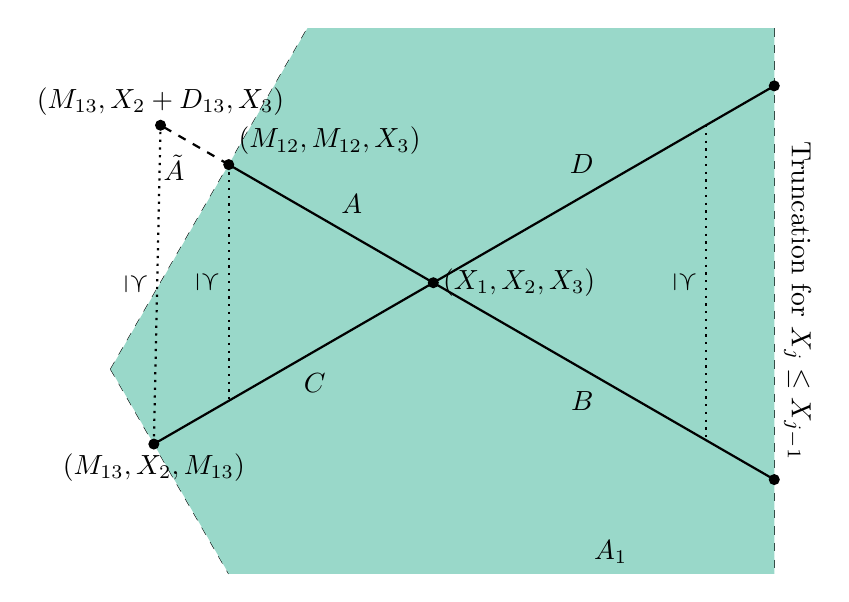
\begin{tikzpicture}
	\coordinate (C1) at (60:5);
	\coordinate (C2) at (300:3);
	\coordinate (A) at (60:3);
	\coordinate (B) at ($(A) + (330:3)$);
	\coordinate (C) at ($(0, 0)!(B)!(C2)$);
	\coordinate (D) at ($(A) + (150:1)$);
	\coordinate (C3) at ($(B) + (330:5)$);
	\coordinate (C4) at ($(B) + (30:5)$);
	\coordinate (C5) at ($(C3)!(C1)!(C4)$);
	\coordinate (C6) at ($(C3)!(C2)!(C4)$);
	\draw[dashed] (0, 0) -- (C1);
	\draw[dashed] (0, 0) -- (C2);
	\draw[dashed] (C5) -- (C6) node[midway, above, rotate = -90] {Truncation for $X_j \le X_{j-1}$};
	\fill[mid_green] (0, 0) -- (C1) -- (C5) -- (C6) -- (C2) -- cycle;
	\node[above] at ($(C2)!0.7!(C6)$) {$A_1$};
	\draw[thick] (A) -- (B) node[midway, above right] {$A$};
	\draw[thick] (B) -- (C3) node[midway, below left] {$B$};
	\fill (C3) circle(2pt);
	\fill (A) circle(2pt) node[above right] {$\left(M_{12}, M_{12}, X_3\right)$};
	\fill (B) circle(2pt) node[right] {$\left(X_1, X_2, X_3\right)$};
	\draw[thick] (C) -- (B) node[midway, below right] {$C$};
	\node[below] at (C) {$\left(M_{13}, X_2, M_{13}\right)$};
	\draw[thick] (B) -- (C4) node[midway, above left] {$D$};
	\fill (C4) circle(2pt);
	\fill ($(0, 0)!(B)!(C2)$) circle(2pt);
	\draw[thick, dashed] (A) -- (D) node[midway, below left] {$\tilde{A}$};
	\fill (D) circle(2pt) node[above] {$\left(M_{13}, X_2 + D_{13}, X_3\right)$};
	\draw[thick, dotted] (C) -- (D) node[midway, below, rotate=-90] {$\succeq$};
	\draw[thick, dotted] (A) -- ++(0, -3) node[midway, below, rotate=-90] {$\succeq$};
	\draw[thick, dotted] ($(B) + (30:4)$) -- ($(B) + (330:4)$) node[midway, below, rotate=-90] {$\succeq$};
\end{tikzpicture}
\end{center}
\caption{The two $p$-values constructed corresponds to taking integrals of $g$ along these segments, that lie on a level set of $x_j + x_{j+1} + x_k$. The dashed line corresponds to extension in \Cref{eqn:int_extension}. The dotted line on the far right is the truncation that enforces $X_j < X_{j-1}$.}
\label{fig:crop_rays}
\end{figure}

Here we are only comparing $X_j$ to $X_{j+1}$ by \Cref{sec:winnerbest}. The upper truncation for $X_j$ can be represented by cropping \Cref{fig:compare_rays} along a vertical line, shown in \Cref{fig:crop_rays}, thus the proof of Part 1 of \Cref{thm:main} that it suffices to compare $X_1$ and $X_2$ remains valid with appropriate conditioning. Again we can construct the $p$-values as in \Cref{eqn:p1j} for $k>j$.

$$p_{jk} = \frac{\int_{D_{jk}}^{X_{j-1}} g\left(X_1, \ldots, M_{jk} + z, \ldots, M_{jk} - z, \ldots, X_n\right) \,dz}{\int_{\max\left\{X_{j+1} - M_{jk}, 0\right\}}^{X_{j-1}} g\left(X_1, \ldots, M_{jk} + z, \ldots, M_{jk} - z, \ldots, X_n\right) \,dz}.$$

Hence similar to the proof of Part 1 of \Cref{thm:main}, Schur-concavity ensures $p_{j\left(j+1\right)} \ge p_{jk}$ for all $k>j$, meaning that it is sufficient to compare $X_j$ and $X_{j+1}$. In fact, we can take $p_j = p_{j\left(j+1\right)}$. These are valid selective $p$-value as required in \citet{Fithian:2015uj}, as
\begin{align*}
\PP_\theta \left[p_j \le \alpha \mid \theta_{[k]} \text{ is not the } k\text{-th largest, for some } k \le j\right] = \PP_\theta \left[p_j \le \alpha \mid \mathcal{M}_j\left(X\right)^c = M\right] \le \alpha \text{ a.s.},
\end{align*}
for all $\theta \in M$, where $M$ is the selected model, by tower property. Note that the conditioning is indeed a random event as the order of $\theta$ depends on $X$ (emphasized with the square brackets here).

The conditioning above indeed holds some significance. The sufficient filtration \citep{Fithian:2015uj} $\mathscr{F}_k$ is given as the $\sigma$-field
\begin{align*}
\mathscr{F}_k & = \sigma\left(\mathcal{M}_0\left(X\right), \ldots, \mathcal{M}_j\left(X\right), X_1, \ldots, X_{j-1}, \frac{X_j + X_{j+1}}{2}, X_{j+2}, \ldots, X_n\right) \\
& = \sigma\left(\left\{X_1 > \ldots > X_j > \max_{k>j} X_k\right\}, X_1, \ldots, X_{j-1}, \frac{X_j + X_{j+1}}{2}, X_{j+2}, \ldots, X_n\right) \\
& = \sigma\left(\mathcal{M}_j\left(X\right), X_1, \ldots, X_{j-1}, \frac{X_j + X_{j+1}}{2}, X_{j+2}, \ldots, X_n\right),
\end{align*}
which is the conditioning we used just now. Hence the nested sequence of model satisfies the subpath sufficiency principle , and the $p$-values sequence $p_j$ is independent on nulls, as defined in and shown in Theorem 4 of \citet{Fithian:2015uj}. Thus the step-down procedure where we keep rejecting $H_{0j}$ until the first time that $p_j > \alpha$ controls FWER.

\WFcomment{Should the reference to SSP be earlier if you are going to say it? Also, is it actually necessary to bring up the SSP? You've already said directly that we are conditioning on $X_{[1]}$ through $X_{[j-1]}$. More generally, if we can sidestep the more generic langauge of that paper and substitute more specific language for our specific problem, I think that will make this a lot more readable.}
\end{proof}

\begin{customthm}[Part 3 of \Cref{thm:main}]
Assume the model~\eqref{eqn:expfam} holds and $g\left(x\right)$ is a Schur-concave function. Procedure 3 is a conservative step-down procedure with FWER no larger than $\alpha$.
\end{customthm}

\begin{proof}
The $p$-values $p_{j\left(j+1\right)}$ obtained in Procedure 3' are always smaller than their counterpart in Procedure 3, as the upper truncation at $X_{j-1}$ is on the upper tail. Therefore Procedure 3 is conservative and definitely valid.
\end{proof}

\section{Discussion}
\label{sec:disc}

\WFcomment{Discussion still needs fleshing out.}

Our selective test procedure allows us to untangle multiple comparisons based on correlated observations easily, while avoiding the pitfalls of selection. Claims reporting the ``winner'' are commonly made in the scientific literature, usually with no significance level reported or an incorrect method applied. For example, \citet{Uhls:2012gf} asked $n=20$ elementary and middle school students which of seven personal values they most hoped to embody as adults: ``Fame'' (8 selected), ``Benevolence'' (5), ``Achievement'' (3), and several others (4 total including one response of ``Other''). The authors' main finding --- which appeared in the abstract, the first paragraph of the article, and later a CNN.com headline --- was that ``Fame'' was the most common response. This claim was accompanied by a significance level of $0.006$, which the authors computed by testing whether the probability of selecting ``Fame'' was larger than 1/7.

The obvious error in the authors' reasoning is perhaps understandable since there is, presently, no agreed-upon statistical solution for this commonplace problem. Using our approach, they could have performed a two-tailed binomial test of the winner (``Fame'') vs. the runner-up (``Benevolence''). This test returns a $p$-value of
$$p = 2 \cdot \PP\left[\text{Binomial}\left(8 + 5, 0.5\right) \ge 8\right] = 0.58,$$
indicating that their data did not support their major finding.

This paper has provided a straightforward yet powerful method for verifying that the winner is the best, for joint distributions in the exponential family with a mild technical condition. Such a test allows us to ``ignore'' the issues of selection and multiple-testing with relative ease and power. \WFcomment{This last sentence might give the wrong impression.}

\bibliographystyle{plainnat}
\bibliography{papers,additional}

\end{document}